  Para la última etapa se utiliza la gramática de atributos para definir
semántica sobre el \emph{AST}.

Las gramáticas de atributos (\emph{Attribute Grammars}
\cite{attributegrammars} \cite{uuag}) simplifican
la tarea de escribir catamorfismos.
Un catamorfismo es una función análoga a la función de alto orden
\texttt{foldr} pero aplicada sobre cualquier tipo de datos recursivo.

  De ésta manera se pueden definir atributos sintetizados,
  heredados o mixtos en el \emph{AST}.

  Los atributos sintetizados son valores que se distribuyen desde las
hojas hacia la raiz del \emph{AST}, y los heredados aquellos que
se distribuyen desde la raiz hacia las hojas.

  Uno de dichos atributos será el código en bajo nivel, la salida
de esta etapa.

  Se implementó una gramática de atributos usando \textit{UUAG}, y con
  el compilador de gramáticas \textit{UUAGC}\cite{uuagc} se
  compiló a \haskell{}.

  El compilador \textit{UUAGC} toma la gramática y construye los
  catamorfismos necesarios para procesar todos los atributos.

  Construir el compilador, se reduce a obtener una secuencia de atributos
  sobre el \textit{AST} que sirven para generar el código \alf{}.

  Por ejemplo para construir el código de un programa, la raiz
  del \textit{AST} está dada por el tipo de datos \texttt{Root}.

\begin{Verbatim}
data Root
  | Root
      decls :: Decls
      dodecls :: Dodecls
\end{Verbatim}

  Se puede definir el código como la concatenación del código de
  las declaraciones del bloque \texttt{do}, una instrucción \texttt{halt}
  y el código de las declaraciones de funciones (\texttt{Decls}).

  Para ésto se define un atributo sintetizado (\texttt{syn})
  llamado \texttt{code}.


\begin{Verbatim}
set All = Root Decls Decl Dodecls Dodecl Expr
attr All syn code use {++} {[]} :: BC

sem Root
  | Root
    lhs.code = @dodecls.code ++ [Thalt] ++ @decls.code
\end{Verbatim}

  Utilizando la palabra clave \texttt{Set} se define el conjunto \texttt{All}
de elementos para los que se definirá el atributo.
  
  En la definición del atributo, se especifica que en caso de no haber
una regla específica, se calcula usando la concatenación \texttt{++}
y como atributo por defecto toma \texttt{[]}. A ésto se le llama
\textit{use rule}.

  \begin{Verbatim}
  attr All syn code use {++} {[]} :: BC
  \end{Verbatim}

  Por ejemplo para la definición de la lista de declaraciones:

\begin{Verbatim}
type Decls = [Decl]
\end{Verbatim}

  No es necesario especificar que el código se obtiene concatenando sus
  partes ya que se infiere automáticamente usando la regla anterior.


  Para poder generar el código de todo el programa, es necesario
  calcular otros atributos previos.
  Se necesita saber la posición en la que quedarán las funciones para
  poder tener una referencia a ellas.
  Para saber la posición, es necesario calcular el largo del código
  antes de tener el código.

  Para ésto se definió un atributo sintetizado \texttt{len} que contiene
  el largo que tendrá cada bloque luego de traducido
  a código, pero sin llegar a traducirlo.

  También se definió un atributo \texttt{pos} que indica en que posición
  estará ubicado el código que se genere para cada producción de la
  gramática.
  El atributo \texttt{pos} es un atributo heredado (\texttt{inh}) en
  el \textit{AST}.

  Por ejemplo en \texttt{Root}, se utiliza el atributo \texttt{len} 
  de las declaraciones del bloque \texttt{do} para saber a partir
  de que posición \texttt{pos} estarán ubicadas las declaraciones
  de funciones.

\begin{Verbatim}
attr All syn code use {++} {[]} :: BC
         syn len use {+} {0} :: Int
         inh pos :: Int
 
sem Root
  | Root
      lhs.code = @dodecls.code ++ [Thalt] ++ @decls.code
      dodecls.pos = 0
      decls.pos = @dodecls.len + 1
\end{Verbatim}

  Utilizando el atributo \texttt{pos}, se puede saber en que posición
  estará cada función en el código generado.
  Para tener la posición de todas las funciones se utiliza un atributo
  encadenado (\texttt{chn}) llamado \texttt{labels},
  es heredado pero también es sintetizado.
  Por ejemplo al declarar una función, se agrega la posición \texttt{pos}
  asociada al nombre de la misma.

\begin{Verbatim}
sem Decl
  | Function
      lhs.code = @body.code ++ [Tret]
      lhs.len = @body.len + 1
      lhs.labels = addLabel @name @lhs.pos @lhs.labels
\end{Verbatim}

  El atributo contiene un mapa que dado un nombre de una función retorna
  la posición de la misma, \texttt{labels} recolecta la posición de todas
  las funciones.
  Luego otro atributo \texttt{labelMap} se declara como heredado \texttt{inh}
  y se le asigna en \texttt{Root} el valor de \texttt{labels},
  \texttt{labelMap} se usa para distribuir el mapa
  completo en todo el \textit{AST}.

\begin{Verbatim}
sem Root
  | Root
      decls.labels = emptyLabelMap
      decls.labelMap = @decls.labels
      dodecls.labelMap = @decls.labels
\end{Verbatim}

  Por último un atributo \texttt{env} encadenado recolecta las declaraciones
  de identificadores, a cada identificador de señal le asigna un número
  entero único y mantiene la lista de las variables en el alcance (scope)
  dentro de una función. 
  Luego que el atributo \texttt{env} recolecta todas las declaraciones,
  el resultado es distribuido con el atributo heredado \texttt{envInh}.

\begin{Verbatim}
sem Root
  | Root
      decls.env = emptyEnv
      dodecls.env = emptyEnv
      dodecls.envInh = @dodecls.env
\end{Verbatim}

  Usando todos éstos atributos se genera el código para cada producción
  de la gramática, y el atributo \texttt{code} se puede calcular.

  Se definió un módulo \texttt{Bytecode} que abstrae el código
  de máquina en un tipo \texttt{OpCode} y define funciones para 
  exportarlo como texto o en formato binario.


  Al compilar la gramática usando \textit{UUAGC} se obtiene un módulo
  en lenguaje \texttt{Haskell} que expone la función \texttt{code\_Syn\_Root}
  y deja accesible el código resultado como una lista de
  tipo \texttt{[OpCode]}.

  Utilizando el módulo \texttt{Bytecode}, el código se obtiene y 
escribe en un archivo (.alf) terminando el proceso de compilación.

  Los módulos del compilador y sus dependencias se pueden ver en
la Figura \ref{fig:williecmodules}.

\begin{figure}[h!]
  \begin{center}
    \caption{Paquetes del compilador \compilador{}}
    {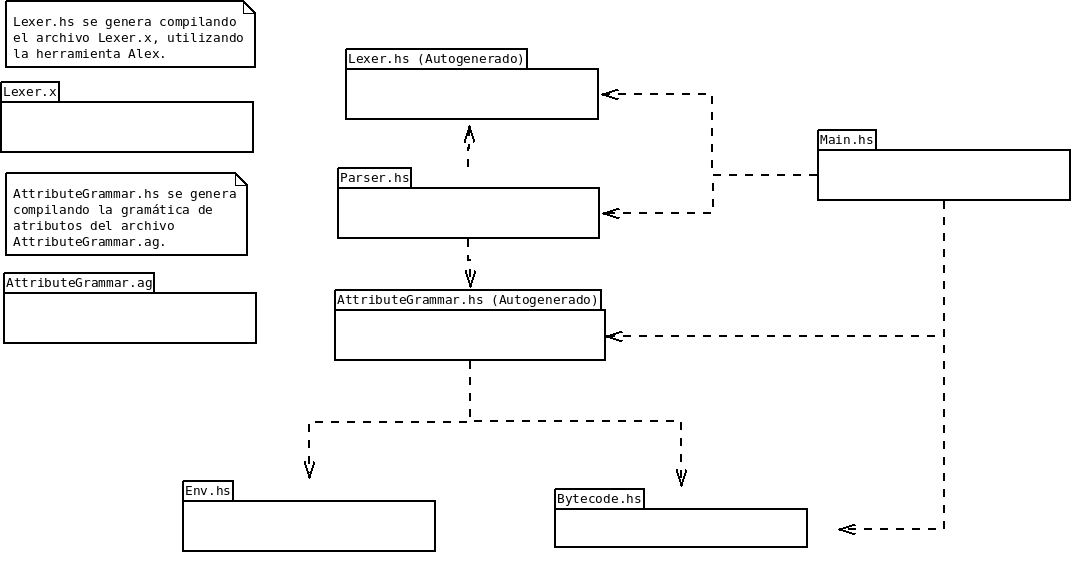
\includegraphics[width=160mm]{graphs/williecpackages.png}}
   \label{fig:williecmodules}
  \end{center}
\end{figure}
